\documentclass[11pt]{beamer}

\usetheme{metropolis}

\usepackage{graphicx}
\usepackage{physics}
\usepackage{adjustbox}
\usepackage{caption}
\usepackage{chemformula}
\usepackage{quoting}
\usepackage[style=chem-angew,backend=bibtex]{biblatex}
\bibliography{references}
%
% Choose how your presentation looks.
%
% For more themes, color themes and font themes, see:
% http://deic.uab.es/~iblanes/beamer_gallery/index_by_theme.html
%
\mode<presentation>
{
  \usetheme{default}      % or try Darmstadt, Madrid, Warsaw, ...
  \usecolortheme{default} % or try albatross, beaver, crane, ...
  \usefonttheme{default}  % or try serif, structurebold, ...
  \setbeamertemplate{navigation symbols}{}
  \setbeamertemplate{caption}[numbered]
  \setbeamerfont{footnote}{size=\tiny}
} 

\usepackage[english]{babel}
\usepackage[utf8]{inputenc}
\graphicspath{{../lectureMW/image/}}

\AtBeginSection[]{
\begin{frame}{Outline}
  \tableofcontents[currentsection]
\end{frame}
}

\title{Chapter 2: Atoms, Ions, and the Periodic Table}
\institute{Chemistry Department, Cypress College}
\date{August 29, 2022}

\begin{document}

\begin{frame}
  \titlepage
\end{frame}

\begin{frame}{Lecture Weekly Agenda}
  \begin{itemize}
  \item Cover Ch 1 - pg $1 - 55$
  \item Go over Ch 2 - pg $56 - 88$
  \item In-class Ch 1+2 worksheet
  \item First class quiz released Fri, Sept 2nd at 11am
  \end{itemize}
\end{frame}

\begin{frame}{Correction to Lecture 3}
  \centering
  \includegraphics[scale=0.15]{water}

  \begin{itemize}
  \item Water is a pure substance
  \end{itemize}
\end{frame}

\section{Review: Scientific Method and Atoms}

\begin{frame}{Review: Scientific Method}
  \begin{enumerate}
  \item Gather observations
  \item Ask a question. Propose a hypothesis
    which is a supposed explanation of a given phenomenon
  \item Design and perform your experiment
  \item If results support the hypothesis, then propose
    a theory, which explains the observation. If not, then revise
    the hypothesis.
  \end{enumerate}
\end{frame}

\begin{frame}{What are atoms made of?}
  \centering
  \begin{tabular}{c|ccc}
    & Mass (g) & Atomic Units (Amu) & Charge (C) \\
    \hline
    Neutron  & $1.675\times 10^{-24}$ & 1 & 0 \\
    Proton   & $1.675\times 10^{-24}$ & 1 & $1.6022\times 10^{-19}$ \\
    Electron & $9.1094\times 10^{-28}$ & 1/1840 & $-1.6022\times 10^{-19}$
  \end{tabular}

  \begin{itemize}
  \item 1 amu = $1.6606 \times 10^{-24}$ g
  \item Protons and neutrons are located in the nucleus
  \item Electrons revolve around the nucleus (difference between
    core electrons and valence electrons)
  \end{itemize}
\end{frame}

\section{Periodic Table - Grouped Elements}

\begin{frame}{Earliest Periodic Table}
  \begin{center}
    \includegraphics[scale=0.13]{mendeleev_table}
  \end{center}
  
  \begin{itemize}
  \item Dmitrij Mendeleev Arranged base on atomic mass
  \item Grouped known elements into rows and columns
  \end{itemize}
\end{frame}

\begin{frame}{Modern Period Table}
  \centering
  \includegraphics[width=\linewidth]{ptable}
\end{frame}

\begin{frame}{Mass Spectroscopy: Determining the Atomic Mass}
  \begin{center}
    \includegraphics[width=\linewidth]{mass_spect}
  \end{center}

  \begin{itemize}
  \item Ionizes the atom and electric field accelerates atoms
  \item Time of flight - heavier atoms will travel slower
    than lighter ones
  \item Weighter average of atomic masses
  \end{itemize}
\end{frame}

\begin{frame}{Relative Atomic Mass Formula}
  \begin{equation}
    \text{Relative Atomic Mass} = (I_1\times A_1) + (I_2\times A_2) + \dots
  \end{equation}
  where $I$ is the mass of the isotope, and $A$ is the
  relative abundance between 0 and 1
\end{frame}

\begin{frame}{Calculating the Relative Atomic Masses}
  Magnesium is composed of three isotopes. Calculate the
  relative atomic mass of magnesium and compare to the periodic
  table.
  \begin{center}
  \begin{tabular}{ccc}
    Isotope & Mass (amu) & Natural Abundance ($\%$) \\
    \hline
    $^{24}$Mg & 23.985 & 78.99 \\
    $^{25}$Mg & 24.986 & 10.00 \\
    $^{26}$Mg & 25.983 & 11.01
  \end{tabular}
  \end{center}
\end{frame}

\begin{frame}{Calculating the Relative Atomic Masses}
  Magnesium is composed of three isotopes. Calculate the
  relative atomic mass of magnesium and compare to the periodic
  table.
  \begin{center}
  \begin{tabular}{ccc}
    Isotope & Mass (amu) & Natural Abundance ($\%$) \\
    \hline
    $^{24}$Mg & 23.985 & 78.99 \\
    $^{25}$Mg & 24.986 & 10.00 \\
    $^{26}$Mg & 25.983 & 11.01
  \end{tabular}
  \end{center}

  \begin{align*}
    23.985\text{amu}\times 0.7899 & =  18.95 \text{amu} \\
    24,986\text{amu}\times 0.1000 & =  2.499 \text{amu} \\
    25.983\text{amu}\times 0.1101 & =  2.861 \text{amu} \\
    \hline
    &   24.31 \text{amu}
  \end{align*}
\end{frame}

\begin{frame}{Practice: Calculate the Atomic Mass}
  Boron has two naturally occuring isotopes. Determine the
  atomic mass of boron.
  
  \begin{center}
  \begin{tabular}{cc}
    Isotope & Natural Abundance ($\%$) \\
    \hline
    $^{10}$B & 19.9 \\
    $^{11}$B & 80.1 
  \end{tabular}
  \end{center}
\end{frame}

\begin{frame}{Practice: Calculate the Atomic Mass}
  \begin{center}
    \includegraphics[scale=0.175]{cl_mass_spec}
  \end{center}
  Determine atomic mass of Cl given the mass spectrum. Hint:
  Cl naturally exists as a diatomic e.g. Cl$_2$.
\end{frame}

\begin{frame}{Conceptual Question}
  Naturally occurring gallium (ga) is made of two isotopes
  Ga-69 and Ga-71. Which of the following statements is true?
  Hint: Look at the periodic table.
  
  \begin{enumerate}
  \item Gallium's relative atomic mass is 70.00 amu
  \item Both isotopes have the same mass: 69.72 amu
  \item The isotopes are present in the same percentages
  \item Ga-71 is present in the largest percent abundance
  \item Ga-69 is present in the largest percent abundance
  \end{enumerate}
\end{frame}

\begin{frame}{Alkali Metal}
  \begin{center}
    \includegraphics[scale=0.2]{alkali_metal}
  \end{center}
  
  \begin{itemize}
  \item Lower densities than other metals
  \item Extremely soft metals
  \item Highly reactive e.g. forming H$_2$ when in
    contact with water
  \item Prefer to lose an electron
  \end{itemize}
\end{frame}

\begin{frame}{Alkaline Earth Metal}
  \begin{center}
    \includegraphics[width=0.4\linewidth]{alkaline_metal}
  \end{center}
  
  \begin{itemize}
  \item Fairly reactive metals
  \item Can form solutions with a pH greater than
    7 (more basic or alkaline)
  \item Calcium and magnesium important for life
  \item Prefer to lose 2 electrons
  \end{itemize}
\end{frame}

\begin{frame}{Transition Metals}
  \begin{center}
    \includegraphics[scale=0.12]{copper_pan}
  \end{center}
  
  \begin{itemize}
  \item Easily malleable and great conductors of heat and
    electricity
  \item High melting points except mercury (liquid at Room
    temperature)
  \item High densities
  \item Oxidation states (ability to gain/lose electrons) can
    vary between 1+ to 6+
  \end{itemize}
\end{frame}

\begin{frame}{Actinides and Lanthanides}
  \begin{center}
    \includegraphics[scale=0.3]{quantum_comp}
  \end{center}

  \begin{itemize}
  \item Radioactive due to instability
  \item Silvery/silvery-white luster in metallic form
  \item Potential application to quantum computers and
    nuclear power
  \item Oxidation states can range from 2+ to 7+
  \end{itemize}
\end{frame}

\begin{frame}{Materials for Quantum Computing: Lanthanide Complexes}
  \begin{columns}
    \column{0.4\textwidth}
    \centering
    \includegraphics[scale=0.15]{gd_homo}
    \textbf{[1-Gd]$^{-1}$} HOMO
    
    \column{0.7\textwidth}
    \centering
    \includegraphics[scale=0.14]{gd_uv}
  \end{columns}

  \begin{itemize}
  \item Understanding the electronic structure
  \item Hysteresis - electronic spin memory
  \item \href{https://pubs.acs.org/doi/10.1021/jacs.1c03098}
    {Lanthanide MoS$_4$ research article}
  \end{itemize}
\end{frame}

\begin{frame}{Nuclear Power Plants}
  \begin{center}
    \includegraphics[width=\linewidth]{nuclear_plant}
  \end{center}
\end{frame}

\begin{frame}{Halogens}
  \begin{itemize}
  \item Fairly toxic and form acids when combined with
    hydrogen
  \item Readily react with metals to form salts e.g.
    NaCl
  \item Important for drug development due to their ``sticky''
    nature
  \item Prefers to gain an electron
  \end{itemize}
\end{frame}

\begin{frame}{Cancer Therapeutics}
  \vspace*{0.5cm}
  \begin{columns}
    \column{0.6\textwidth}
    \centering
    \includegraphics[width=0.7\linewidth]{sea_squirt}
    %\vspace*{-0.35cm}
    \hspace*{-1cm}
    \column{0.5\textwidth}
    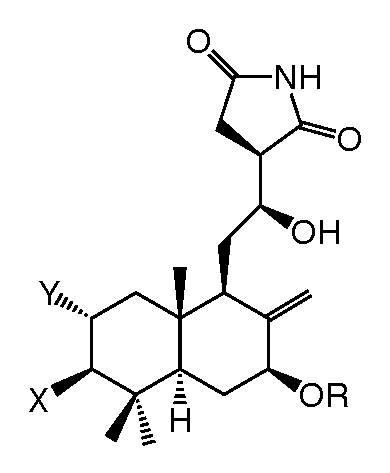
\includegraphics[width=0.4\linewidth]{lisso_struct}
    \begin{table}
      \scalebox{0.75}{
        \begin{tabular}{l|ccc}
          \hline
          Compound & X & Y & R \\
          \hline\hline
          Chlorolissoclimide (CL)   & H  & Cl & H \\
          Dichlorolissoclimide (DCL)& Cl & Cl & H \\
          \hline
        \end{tabular}
      }
    \end{table}
  \end{columns}

  \begin{itemize}
  \item Chlorolissoclimide is a potent cancer drug that
    is naturally found in sea squirts
  \item Understanding the structure--activity relationships
    e.g. interactions between drug and ribosome
  \end{itemize}
\end{frame}

\begin{frame}{My Research Project: Chlorolissoclimide}
  \begin{center}
    \includegraphics[trim={0 4.2in 0 0},clip,scale=0.4]{lisso_drug}
  \end{center}

  \begin{itemize}
  \item \href{https://www.nature.com/articles/nchem.2800}
    {Chlorolissoclimide research article}
  \end{itemize}
\end{frame}

\begin{frame}{Noble Gases}
  \begin{center}
    \includegraphics[scale=0.7]{neon_lights}
  \end{center}
  
  \begin{itemize}
  \item Colorless, odorless, tasteless, and non-flammable
    under standard conditions
  \item Extremely non-reactive and most stable elements
  \item Do not like to gain or lose electrons
  \end{itemize}
\end{frame}

\begin{frame}{Practice: Periodic Table}
  Group the elements into the following groups
  \begin{itemize}
  \item Br
  \item K
  \item Mg
  \item Al
  \item Mn
  \item Ar
  \item U
  \end{itemize}
\end{frame}

\begin{frame}{Practice}
  What is the charge of the ions for each of the following elements?

  \begin{itemize}
  \item Al
  \item P
  \item Br
  \item S
  \end{itemize}
\end{frame}

\end{document}
